% OrbitalNet OS — illustrated handout. Build: bash docs/handout/build.sh
% No result number is typed here: all come from numbers.tex / vars.tex (generated).
\documentclass[9.5pt]{article}
\usepackage[a4paper,left=11mm,right=11mm,top=11mm,bottom=12mm]{geometry}
\usepackage[T1]{fontenc}
\usepackage[scaled]{helvet}
\renewcommand{\familydefault}{\sfdefault}
\usepackage{amsmath,amssymb}
\usepackage{multicol}
\usepackage[dvipsnames]{xcolor}
\usepackage{tikz}
\usetikzlibrary{shadings,arrows.meta,calc,positioning,decorations.pathmorphing,fadings}
\usepackage[most]{tcolorbox}
\usepackage{pgfplots}\pgfplotsset{compat=1.17}\usepgfplotslibrary{fillbetween}
\usepackage{enumitem}
\usepackage{titlesec}
\usepackage{pifont}
% GENERATED by research/figures/paper_main.py -- do not edit
\newcommand{\CausalBugPct}{98\%}
\newcommand{\SimGamma}{0.1}
\newcommand{\SimLengthscale}{1.2}
\newcommand{\SimNEvents}{1000}
\newcommand{\SimNModeled}{587}
\newcommand{\SimNWithheld}{413}
\newcommand{\SimHOneVerdict}{\textbf{fail}}
\newcommand{\SimHTwoVerdict}{\textbf{pass}}
\newcommand{\SimHThreeVerdict}{\textbf{pass}}
\newcommand{\SimTtiP}{23.0\,h}
\newcommand{\SimIdP}{99\%}
\newcommand{\SimTtiBzero}{$>$\,budget}
\newcommand{\SimIdBzero}{48\%}
\newcommand{\SimHolmBzero}{$<10^{-4}$}
\newcommand{\SimRbcBzero}{0.52}
\newcommand{\SimFasterBzero}{50\%}
\newcommand{\SimSlowerBzero}{48\%}
\newcommand{\SimTtiBone}{12.05\,d}
\newcommand{\SimIdBone}{61\%}
\newcommand{\SimHolmBone}{$<10^{-4}$}
\newcommand{\SimRbcBone}{0.63}
\newcommand{\SimFasterBone}{62\%}
\newcommand{\SimSlowerBone}{27\%}
\newcommand{\SimTtiBtwo}{13.8\,h}
\newcommand{\SimIdBtwo}{72\%}
\newcommand{\SimHolmBtwo}{0.00019}
\newcommand{\SimRbcBtwo}{0.19}
\newcommand{\SimFasterBtwo}{30\%}
\newcommand{\SimSlowerBtwo}{49\%}
\newcommand{\SimTtiBthree}{1.59\,d}
\newcommand{\SimIdBthree}{99\%}
\newcommand{\SimHolmBthree}{$<10^{-4}$}
\newcommand{\SimRbcBthree}{0.33}
\newcommand{\SimFasterBthree}{48\%}
\newcommand{\SimSlowerBthree}{25\%}
\newcommand{\SimObsP}{4.2}
\newcommand{\SimObsBthree}{2.9}
\newcommand{\SimHtwoFast}{0.414}
\newcommand{\SimHtwoSlow}{0.152}
\newcommand{\SimHtwoEst}{0.261}
\newcommand{\SimHtwoCI}{[0.153, 0.368]}
\newcommand{\SimHtwoFastCI}{[0.314, 0.514]}
\newcommand{\SimHtwoSlowCI}{[0.113, 0.195]}
\newcommand{\SimTprP}{96\%}
\newcommand{\SimTprBthree}{21\%}
\newcommand{\SimHthreeEst}{76}
\newcommand{\SimHthreeCI}{[66, 84]}
\newcommand{\SimAucP}{0.993}
\newcommand{\SimAucBthree}{0.666}
\newcommand{\SimAucBtwo}{0.696}
\newcommand{\SimAucPown}{0.714}
\newcommand{\SimTprPown}{21\%}
\newcommand{\SimCwWhBthree}{97\%}
\newcommand{\SimCwWhP}{6\%}
\newcommand{\SimAccModP}{100\%}
\newcommand{\SimAccModBthree}{100\%}
\newcommand{\SimFaP}{0\%}
\newcommand{\SimFaPModelError}{13\%}
\newcommand{\SimAccModPModelError}{87\%}
\newcommand{\SimAucPModelError}{0.891}
\newcommand{\SimAucBthreeModelError}{0.706}
\newcommand{\SimAucPCrowding}{0.975}
\newcommand{\SimObsAllP}{4.2}
\newcommand{\SimAccModPAll}{100\%}
\newcommand{\SimCwWhPAll}{6\%}
\newcommand{\SimFlagP}{89\%}
\newcommand{\SimAucAblP}{0.993}
\newcommand{\SimObsAllNoDecay}{3.6}
\newcommand{\SimAccModNoDecayAll}{99\%}
\newcommand{\SimCwWhNoDecayAll}{31\%}
\newcommand{\SimFlagNoDecay}{65\%}
\newcommand{\SimAucAblNoDecay}{0.936}
\newcommand{\SimObsAllNoAdeq}{4.3}
\newcommand{\SimAccModNoAdeqAll}{100\%}
\newcommand{\SimCwWhNoAdeqAll}{6\%}
\newcommand{\SimFlagNoAdeq}{89\%}
\newcommand{\SimAucAblNoAdeq}{0.992}
\newcommand{\SimObsAllBthree}{2.8}
\newcommand{\SimAccModBthreeAll}{100\%}
\newcommand{\SimCwWhBthreeAll}{97\%}
\newcommand{\SimObsAllBtwo}{4.9}
\newcommand{\SimAccModBtwoAll}{88\%}
\newcommand{\SimCwWhBtwoAll}{69\%}
\newcommand{\SimObsAllBone}{3.2}
\newcommand{\SimAccModBoneAll}{80\%}
\newcommand{\SimCwWhBoneAll}{75\%}
\newcommand{\SimObsAllBzero}{5.0}
\newcommand{\SimAccModBzeroAll}{79\%}
\newcommand{\SimCwWhBzeroAll}{1\%}
\newcommand{\SimDeltaKilonova}{1.59}
\newcommand{\SimDeltaShock}{0.32}
\newcommand{\SimDeltaFlare}{-0.56}
\newcommand{\SimDeltaGrb}{0.15}
\newcommand{\SimHtwoModelErrorEst}{-0.098}
\newcommand{\SimHtwoModelErrorCI}{[-0.171, -0.024]}
\newcommand{\SimHtwoCrowdingEst}{0.232}
\newcommand{\SimHthreeModelErrorEst}{17}
\newcommand{\SimHthreeModelErrorCI}{[8, 31]}
\newcommand{\SimAccModBthreeModelError}{99\%}
\newcommand{\SimHOneCrowding}{fail}
\newcommand{\SimHTwoCrowding}{pass}
\newcommand{\SimHThreeCrowding}{pass}
\newcommand{\SimHOneModelError}{fail}
\newcommand{\SimHTwoModelError}{fail}
\newcommand{\SimHThreeModelError}{pass}
\newcommand{\RealCHOneVerdict}{\textbf{pass}}
\newcommand{\RealCHTwoVerdict}{\textbf{pass}}
\newcommand{\RealCHThreeVerdict}{\textbf{pass}}
\newcommand{\RealCHFourVerdict}{\textbf{pass}}
\newcommand{\RealCHFiveVerdict}{\textbf{fail}}
\newcommand{\RealRHOneVerdict}{\textbf{pass}}
\newcommand{\RealRHTwoVerdict}{\textbf{pass}}
\newcommand{\RealRHThreeVerdict}{\textbf{fail}}
\newcommand{\RealRHFourVerdict}{\textbf{pass}}
\newcommand{\RealRHFiveVerdict}{\textbf{fail}}
\newcommand{\RealNEvents}{364}
\newcommand{\RealNWithheld}{88}
\newcommand{\RealNModeled}{276}
\newcommand{\RealCAuc}{0.79--0.81}
\newcommand{\RealCCwWhBthree}{50--56\%}
\newcommand{\RealCAccModBthree}{58--62\%}
\newcommand{\RealCCwWhP}{7--14\%}
\newcommand{\RealCAccModP}{59--63\%}
\newcommand{\RealCCwWhBone}{40--45\%}
\newcommand{\RealCAccModBone}{54--56\%}
\newcommand{\RealCFlagP}{39--47\%}
\newcommand{\RealCFaP}{8\%}
\newcommand{\RealRAuc}{0.77--0.80}
\newcommand{\RealRCwWhBthree}{78--80\%}
\newcommand{\RealRAccModBthree}{59--62\%}
\newcommand{\RealRCwWhP}{12--19\%}
\newcommand{\RealRAccModP}{53--54\%}
\newcommand{\RealRCwWhBone}{48--49\%}
\newcommand{\RealRAccModBone}{51--55\%}
\newcommand{\RealRFlagP}{64--73\%}
\newcommand{\RealRFaP}{24--25\%}
\newcommand{\RealCObsP}{2.3}
\newcommand{\RealCObsBthree}{2.6}
\newcommand{\RealCObsBzero}{5.0}
\newcommand{\RealRObsP}{5.0}
\newcommand{\RealRObsBthree}{5.0}
\newcommand{\RealRObsBzero}{5.0}
\newcommand{\ConfAlpha}{0.1}
\newcommand{\ConfAlphaPct}{10\%}
\newcommand{\ConfLambda}{0.25}
\newcommand{\ConfNFresh}{489}
\newcommand{\ConfNCal}{456}
\newcommand{\ConfHCOneVerdict}{\textbf{pass}}
\newcommand{\ConfHCTwoVerdict}{\textbf{pass}}
\newcommand{\ConfHCThreeVerdict}{\textbf{pass}}
\newcommand{\ConfHCFourVerdict}{\textbf{pass}}
\newcommand{\ConfHCFiveVerdict}{\textbf{pass}}
\newcommand{\ConfHCSixVerdict}{\textbf{fail}}
\newcommand{\ConfFa}{3--6\%}
\newcommand{\ConfAccGain}{6--8~points}
\newcommand{\ConfFlag}{42--55\%}
\newcommand{\ConfAucGain}{+0.012--+0.039}
\newcommand{\ConfAccFreshCL}{66--69\%}
\newcommand{\ConfAccFreshP}{61--66\%}
\newcommand{\ConfAccFreshBthree}{60\%}
\newcommand{\ConfAccFreshBthreeConf}{57--58\%}
\newcommand{\ConfRawFaFreshP}{7--9\%}
\newcommand{\ConfCwUnkCL}{26--32\%}
\newcommand{\ConfCwUnkP}{7--14\%}
\newcommand{\ConfCwUnkBthree}{50--56\%}
\newcommand{\ConfFlagBthreeConf}{41--52\%}
\newcommand{\ConfObsP}{2.3--2.4}
\newcommand{\ConfObsL}{3.1--3.2}

\newcommand{\NSat}{10{,}109}
\newcommand{\vSimAucP}{0.993}
\newcommand{\vSimAucBthree}{0.666}
\newcommand{\vSimTprP}{0.960}
\newcommand{\vSimTprBthree}{0.210}
\newcommand{\vSimCwWhP}{0.060}
\newcommand{\vSimCwWhBthree}{0.970}
\newcommand{\vRealCCwWhP}{0.105}
\newcommand{\vRealCCwWhBthree}{0.530}


\definecolor{navy}{HTML}{0B2545}
\definecolor{space}{HTML}{050914}
\definecolor{sky}{HTML}{0EA5E9}
\definecolor{cy}{HTML}{22D3EE}
\definecolor{amb}{HTML}{F59E0B}
\definecolor{grn}{HTML}{16A34A}
\definecolor{rd}{HTML}{DC2626}
\definecolor{vio}{HTML}{7C3AED}
\definecolor{pale}{HTML}{EEF4FB}

\pagestyle{empty}
\setlength{\parindent}{0pt}
\setlength{\parskip}{2pt}
\setlength{\columnsep}{6mm}
\setlength{\columnseprule}{0.3pt}
\def\columnseprulecolor{\color{navy!15}}
\linespread{1.04}

\newcounter{sec}
\newcommand{\sect}[2][sky]{\stepcounter{sec}\vspace{2pt}%
  {\color{#1}\rule[-1.2pt]{2.2pt}{10pt}}\hspace{4pt}{\large\bfseries\color{navy}\thesec.\ #2}\par\vspace{1pt}}

% ── satellite icon ──
\tikzset{
  sat/.pic={
    \fill[pic actions,gray!15,draw=gray!60,line width=.2pt] (-.075,-.06) rectangle (.075,.06);
    \fill[blue!70!cyan,draw=white,line width=.15pt] (-.34,-.05) rectangle (-.11,.05);
    \fill[blue!70!cyan,draw=white,line width=.15pt] (.11,-.05) rectangle (.34,.05);
    \foreach \x in {-.265,-.19,.185,.26} \draw[white,line width=.12pt] (\x,-.05)--(\x,.05);
    \draw[gray!70,line width=.3pt] (-.11,0)--(-.075,0) (.075,0)--(.11,0) (0,.06)--(0,.12);
    \fill[gray!70] (0,.13) circle (.018);
  },
  glow/.style={circle,inner sep=0pt,minimum size=#1},
}
\newcommand{\satglow}[3][cy]{% color, position, scale
  \fill[#1,opacity=.18] #2 circle (.28*#3); \fill[#1,opacity=.28] #2 circle (.17*#3);
  \pic[scale=#3] at #2 {sat};}

\begin{document}
\fontsize{9}{11.2}\selectfont
\setlength{\abovedisplayskip}{3pt}\setlength{\belowdisplayskip}{3pt}\setlength{\abovedisplayshortskip}{2pt}\setlength{\belowdisplayshortskip}{2pt}
% ═════════════════════════ HERO ═════════════════════════
\begin{tikzpicture}[remember picture,overlay]
  \begin{scope}[shift={(current page.north west)}]
  \clip (0,0) rectangle (\paperwidth,-66mm);
  \shade[top color=space,bottom color=navy!80!black] (0,0) rectangle (\paperwidth,-66mm);
  % stars
  \pgfmathsetseed{7}
  \foreach \i in {1,...,230}{\pgfmathsetmacro\sx{rnd*21}\pgfmathsetmacro\sy{-rnd*6.6}\pgfmathsetmacro\so{.25+.7*rnd}
    \fill[white,opacity=\so] (\sx,\sy) circle (.1pt+rnd*.45pt);}
  % sun flare
  \foreach \r/\o in {2.2/.04,1.5/.06,1/.1,.6/.16,.3/.35}{\fill[yellow!60!white,opacity=\o] (19.4,-1.2) circle (\r);}
  \fill[white] (19.4,-1.2) circle (.08);
  % Earth
  \coordinate (E) at (14.2,-31);
  \foreach \r/\o in {25.9/.05,25.6/.08,25.35/.12,25.15/.2}{\fill[cy,opacity=\o] (E) circle (\r);}
  \shade[ball color=blue!65!cyan!80!black] (E) circle (25);
  \fill[navy,opacity=.35] ($(E)+(-3.5,-1)$) circle (24.6);
  % continents-ish blobs
  \begin{scope}\clip (E) circle (25);
    \fill[grn!55!teal,opacity=.55] (10.5,-6.3) .. controls (11.5,-5.6) and (13.2,-5.8) .. (14.1,-6.2) .. controls (14.6,-6.6) and (13,-7) .. (10.5,-6.3);
    \fill[grn!55!teal,opacity=.5] (16.2,-6.1) .. controls (17.4,-5.7) and (19.2,-5.9) .. (20.5,-6.5) -- (20.5,-7) .. controls (18,-6.9) and (17,-6.6) .. (16.2,-6.1);
    \fill[white,opacity=.25] (7,-6.9) .. controls (9,-6.3) and (11,-6.6) .. (12,-6.9) .. controls (10,-7.1) and (8,-7.1) .. (7,-6.9);
    \foreach \a in {68,74,...,110} \draw[white,opacity=.07,line width=.3pt] (E) ++(\a:25) arc (\a:\a+0.0001:25);
  \end{scope}
  % orbits
  \foreach \dr/\c in {.9/cy,1.75/amb,2.6/vio}{
    \draw[\c,opacity=.6,dash pattern=on 1.2pt off 1.8pt,line width=.45pt] (E) ++(67:25+\dr) arc (67:113:25+\dr);}
  % ISL mesh + sats  (ids: c1..c6 inner, a1..a5 middle, v1..v4 outer)
  \foreach \n/\a/\dr in {c1/78/.9,c2/82/.9,c3/86/.9,c4/90/.9,c5/94/.9,c6/98/.9,
                         a1/80/1.75,a2/84.5/1.75,a3/88.5/1.75,a4/93/1.75,a5/97/1.75,
                         v1/83/2.6,v2/87.2/2.6,v3/91.5/2.6,v4/95.5/2.6}{
    \coordinate (\n) at ($(E)+(\a:25+\dr)$);}
  \foreach \p/\q in {c1/c2,c2/c3,c3/c4,c4/c5,c5/c6}{\draw[cy,opacity=.55,line width=.35pt,dashed] (\p)--(\q);}
  \foreach \p/\q in {a1/a2,a2/a3,a3/a4,a4/a5,v1/v2,v2/v3,v3/v4}{\draw[amb,opacity=.5,line width=.35pt,dashed] (\p)--(\q);}
  \foreach \p/\q in {c2/a1,c3/a2,c4/a3,c5/a4,a2/v1,a3/v2,a4/v3}{\draw[white,opacity=.25,line width=.3pt,dashed] (\p)--(\q);}
  % target + enclave beams
  \coordinate (T) at ($(E)+(91.5:25)$);
  \foreach \s in {c4,c5,a3,a4}{\fill[grn,opacity=.12] (\s) -- ($(T)+(-.12,0)$) -- ($(T)+(.12,0)$) -- cycle; \draw[grn,line width=.6pt] (\s)--(T);}
  \foreach \r/\o in {.5/.12,.3/.25,.14/1}{\fill[rd,opacity=\o] (T) circle (\r);}
  \node[white,font=\tiny\bfseries,anchor=west] at ($(T)+(.25,.05)$) {TARGET \,·\, ENCLAVE N=4};
  % ground station RFP beam
  \coordinate (G) at ($(E)+(100.5:25)$);
  \fill[amb] (G) ++(-.08,0) -- ++(.16,0) -- ++(-.08,.14) -- cycle;
  \draw[amb,line width=.6pt,-{Stealth[length=3pt]},decorate,decoration={snake,amplitude=.6pt,segment length=4pt}] (G) -- ($(c6)+(-.05,-.12)$);
  \node[amb,font=\tiny\bfseries,anchor=east] at ($(G)+(-.1,.25)$) {RFP BROADCAST};
  % satellites on top
  \foreach \n/\c in {c1/cy,c2/cy,c3/cy,c4/grn,c5/grn,c6/cy,a1/amb,a2/amb,a3/grn,a4/grn,a5/amb,v1/vio,v2/vio,v3/vio,v4/vio}{
    \satglow[\c]{(\n)}{.62}}
  % title block
  \fill[rd] (1.1,-1.15) rectangle (1.8,-1.22);
  \node[anchor=west,white,opacity=.8,font=\scriptsize\bfseries] at (1.9,-1.18) {MAJOR PROJECT \,·\, SCHOOL OF COMPUTER SCIENCE \& ENGINEERING};
  \node[anchor=north west,white,font=\fontsize{34}{36}\selectfont\bfseries] at (1.0,-1.5) {OrbitalNet OS};
  \node[anchor=north west,cy!40!white,font=\large] at (1.05,-2.9) {Distributed Architecture for Intelligent Satellite Fleet Management};
  \node[anchor=north west,white,font=\small\bfseries] at (1.05,-3.75) {JOYCE MALIK \,·\, MOGHITHA B \,·\, SWATHI SATHISH \,·\, ANUP H \;{\mdseries\color{white!65}(CSE, SCSE)}};
  \end{scope}
\end{tikzpicture}
\vspace*{53.5mm}

% ═════════════════════════ KPI STRIP ═════════════════════════
\newcommand{\kpi}[4]{%
  \begin{tcolorbox}[enhanced,width=.235\textwidth,height=13.5mm,colback=navy,colframe=navy,arc=1.5mm,
     boxrule=0pt,left=2.5mm,right=1mm,top=1.2mm,bottom=0mm,borderline south={1.3pt}{0pt}{#4},valign=center,nobeforeafter,box align=top]
   {\color{white}\fontsize{15}{16}\selectfont\bfseries #1}\\[-1pt]
   {\color{white!80}\fontsize{6.2}{7}\selectfont\bfseries #2}\\[-2pt]{\color{white!55}\fontsize{5.6}{6.5}\selectfont #3}
  \end{tcolorbox}}
\noindent\kpi{\NSat}{SATELLITES IN ORBIT}{real TLEs, SGP4 at 1 Hz}{cy}\hfill
\kpi{\SimAucP}{NOVELTY DETECTION AUROC}{vs \SimAucBthree{} closed-world planner}{grn}\hfill
\kpi{\SimTprP}{NOVEL EVENTS FLAGGED}{vs \SimTprBthree{} baseline, 5\% false alarm}{amb}\hfill
\kpi{\RealNEvents}{REAL ZTF TRANSIENTS}{replayed on the real fleet}{vio}

\vspace{2pt}
\begin{multicols}{2}
% ─────────────────────────────────────────────
\sect[rd]{The Paradigm Shift}
Constellations are growing into the thousands. \textbf{OrbitalNet OS} moves mission intelligence from the ground
to the edge: the ground station simply \emph{announces} intent, and the satellites negotiate among themselves who
serves it, using a Contract Net Protocol (CNP) driven by geometry, energy and health.

\begin{tcolorbox}[enhanced,colback=pale,colframe=navy,boxrule=.5pt,arc=1.5mm,left=2mm,right=2mm,top=1mm,bottom=1mm,
  title={\bfseries Why now?},fonttitle=\footnotesize,colbacktitle=navy,toptitle=.4mm,bottomtitle=.4mm]
\footnotesize
\textbf{Edge compute} on commercial off-the-shelf processors now runs orbital mechanics and consensus on board, and
\textbf{optical inter-satellite links} provide the mesh for real-time negotiation. OrbitalNet OS turns both into a
working fleet operating system.
\end{tcolorbox}

% ─────────────────────────────────────────────
\sect[sky]{How the Fleet Talks}
\begin{center}\vspace{-4pt}
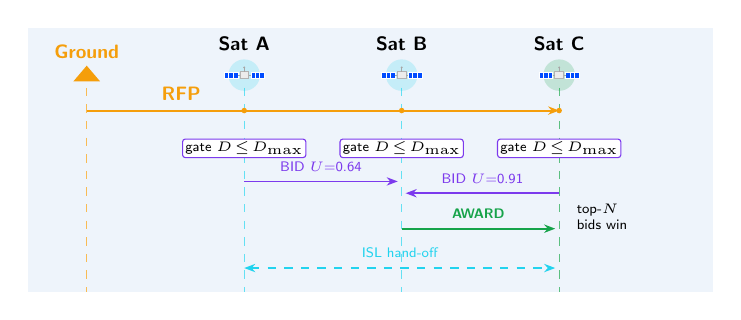
\begin{tikzpicture}[x=1cm,y=1cm,font=\scriptsize]
  \fill[pale] (-.2,-.2) rectangle (8.5,3.15);
  % lanes
  \foreach \x/\n/\c in {.55/Ground/amb,2.55/Sat A/cy,4.55/Sat B/cy,6.55/Sat C/grn}{
     \draw[\c!70,dashed,line width=.4pt] (\x,2.6)--(\x,-.2);}
  \node at (.55,2.85) {\color{amb}\bfseries Ground};
  \fill[amb] (.38,2.47) -- (.72,2.47) -- (.55,2.67) -- cycle;
  \foreach \x/\n/\c in {2.55/A/cy,4.55/B/cy,6.55/C/grn}{
     \fill[\c,opacity=.2] (\x,2.55) circle (.2); \pic[scale=.75] at (\x,2.55) {sat}; \node at (\x,2.95) {\bfseries Sat \n};}
  % messages
  \draw[amb,-{Stealth[length=4pt]},line width=.7pt] (.55,2.1) -- node[above,pos=.2]{\bfseries RFP} (6.55,2.1);
  \foreach \x in {2.55,4.55,6.55}{\fill[amb] (\x,2.1) circle (.035);}
  \foreach \x in {2.55,4.55,6.55}{\node[draw=vio,fill=white,rounded corners=1pt,inner sep=1pt,font=\tiny] at (\x,1.62) {gate $D\!\le\!D_{\max}$};}
  \draw[vio,-{Stealth[length=4pt]},line width=.6pt] (2.55,1.2) -- node[above,font=\tiny]{BID $U$=0.64} (4.5,1.2);
  \draw[vio,-{Stealth[length=4pt]},line width=.6pt] (6.55,1.05) -- node[above,font=\tiny]{BID $U$=0.91} (4.6,1.05);
  \draw[grn,-{Stealth[length=4pt]},line width=.8pt] (4.55,.6) -- node[above,font=\tiny\bfseries]{AWARD} (6.5,.6);
  \draw[cy,{Stealth[length=4pt]}-{Stealth[length=4pt]},line width=.6pt,dashed] (2.55,.1) -- node[above,font=\tiny]{ISL hand-off} (6.5,.1);
  \node[anchor=west,font=\tiny,align=left] at (6.65,.75) {top-$N$\\bids win};
\end{tikzpicture}
\end{center}
\vspace{-6pt}


% ─────────────────────────────────────────────
\sect[vio]{Decision Mathematics}
Each satellite first checks it is in reach of the target with the haversine distance, so only feasible nodes bid:
\begin{equation*}
D = 2R\arcsin\!\sqrt{\sin^2\!\tfrac{\Delta\phi}{2}+\cos\phi_1\cos\phi_2\sin^2\!\tfrac{\Delta\lambda}{2}}\;\le\;D_{\max}
\end{equation*}
Eligible nodes bid a utility blending proximity with battery state of charge; the top-$N$ bids form the enclave:
\begin{equation*}
U=\Big(\frac{D_{\max}-D}{D_{\max}}\Big)w_{\text{prox}} + \text{SoC}\cdot w_{\text{batt}},\qquad
\mathcal{E}=\operatorname{top\text{-}N}\,\{U_i\}
\end{equation*}

% ─────────────────────────────────────────────
\sect[grn]{Rolling Enclaves}
\begin{center}\vspace{-4pt}
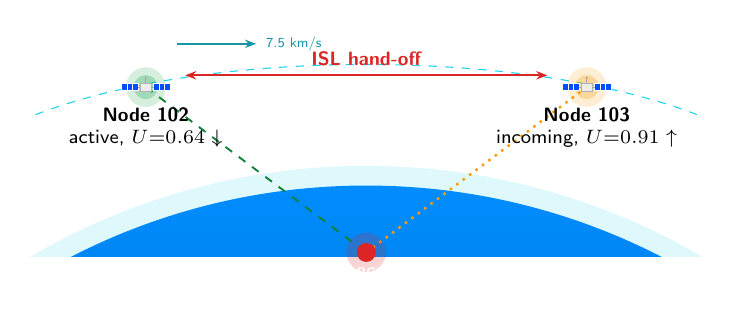
\begin{tikzpicture}[font=\scriptsize]
  \begin{scope}\clip (-.3,-.55) rectangle (8.3,2.3);
    \fill[cy,opacity=.15] (4,-7.85) circle (8.45);
    \shade[top color=blue!45!cyan,bottom color=navy] (4,-7.85) circle (8.2);
  \end{scope}
  \coordinate (T) at (4,-.5);
  \coordinate (A) at (1.2,1.6); \coordinate (B) at (6.8,1.6);
  \draw[cy,dashed,line width=.4pt] (-.2,1.25) .. controls (2,2.1) and (6,2.1) .. (8.2,1.25);
  \draw[grn!80!black,dashed,line width=.7pt] (A)--(T); \draw[amb,dotted,line width=.9pt] (B)--(T);
  \draw[rd,line width=.7pt,{Stealth[length=4pt]}-{Stealth[length=4pt]}] ($(A)+(.5,.15)$) -- node[above]{\bfseries ISL hand-off} ($(B)+(-.5,.15)$);
  \satglow[grn]{(A)}{.9} \satglow[amb]{(B)}{.9}
  \node[below=4pt,align=center] at (A) {\bfseries Node 102 \\ active, $U{=}0.64\downarrow$};
  \node[below=4pt,align=center] at (B) {\bfseries Node 103 \\ incoming, $U{=}0.91\uparrow$};
  \foreach \r/\o in {.25/.2,.12/1}{\fill[rd,opacity=\o] (T) circle (\r);}
  \node[white,below=2pt,font=\tiny\bfseries] at (T) {TARGET};
  \draw[-{Stealth[length=4pt]},cy!70!black,line width=.6pt] (1.6,2.15) -- (2.6,2.15) node[right,font=\tiny]{7.5 km/s};
\end{tikzpicture}
\end{center}
\vspace{-5pt}
Satellites cross the sky at about 7.5\,km/s. As the active node recedes its $U$ falls, the approaching node's $U$
overtakes it, and the enclave hands off automatically: \textbf{coverage that continues and heals itself}.

% ─────────────────────────────────────────────
\sect[rd]{Seeing the Unknown: hypothesis $h_0$}
The fleet also serves science. For a fading astronomical transient, the planner chooses which satellite observes
and when, maximising information gain over known physical models \emph{and} an explicit ``none of the above''
hypothesis $h_0$. Bayesian evidence rewards a model that fits; $h_0$ rises only when none do. No training data is used.
\begin{center}\vspace{-4pt}
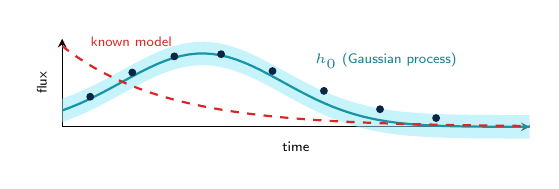
\begin{tikzpicture}
\begin{axis}[width=.62\columnwidth,height=2.7cm,axis lines=left,xlabel={time},ylabel={flux},
  xtick=\empty,ytick=\empty,label style={font=\tiny},xmin=0,xmax=10,ymin=0,ymax=12,clip=false]
  \addplot[name path=up,draw=none,domain=0:10,samples=60] {10*exp(-(x-3)^2/6)+1.6};
  \addplot[name path=lo,draw=none,domain=0:10,samples=60] {10*exp(-(x-3)^2/6)-1.6};
  \addplot[cy!50,opacity=.5] fill between[of=up and lo];
  \addplot[cy!70!black,thick,domain=0:10,samples=60] {10*exp(-(x-3)^2/6)};
  \addplot[rd,thick,dashed,domain=0:10,samples=60] {11*exp(-x/2.2)};
  \addplot[only marks,mark=*,mark size=1.2pt,navy] coordinates {(.6,4.1)(1.5,7.4)(2.4,9.6)(3.4,9.9)(4.5,7.6)(5.6,4.9)(6.8,2.4)(8,1.2)};
  \node[font=\tiny,rd,anchor=west] at (axis cs:0.4,11.6) {known model};
  \node[font=\tiny,cy!60!black,anchor=west] at (axis cs:5.2,9) {$h_0$ (Gaussian process)};
\end{axis}
\end{tikzpicture}\hspace{2mm}%
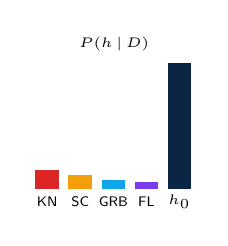
\begin{tikzpicture}[font=\tiny]
  \foreach \i/\h/\l/\c in {0/.25/KN/rd,1/.18/SC/amb,2/.12/GRB/sky,3/.1/FL/vio,4/1.6/$h_0$/navy}{
    \fill[\c] (\i*.42,0) rectangle ++(.3,\h); \node at (\i*.42+.15,-.15) {\l};}
  \node[align=center] at (1,1.85) {$P(h\,|\,D)$};
\end{tikzpicture}
\end{center}
\vspace{-6pt}
{\scriptsize\color{navy!70} Schematic: a known model misfits, $h_0$ fits, and the posterior shifts to $h_0$.}
\begin{equation*}
P(h\mid D)=\frac{p(D\mid h)\,P(h)}{\sum_{h'\in\{h_1,\dots,h_K,\,h_0\}}p(D\mid h')\,P(h')}
\end{equation*}

% ─────────────────────────────────────────────
\sect[amb]{What You Will See in the Demo}
\newcommand{\tile}[3]{\begin{tcolorbox}[enhanced,colback=#1!8,colframe=#1,boxrule=.5pt,arc=1.2mm,left=1.5mm,right=1mm,top=.6mm,bottom=.6mm,
  width=.49\columnwidth,height=8.6mm,valign=center,borderline west={2pt}{0pt}{#1},nobeforeafter]{\scriptsize\bfseries\color{#1!70!black} #2}\par\vspace{-2pt}{\tiny #3}\end{tcolorbox}}
\noindent\tile{sky}{Live 3D globe}{all \NSat{} satellites, streamed to WebGL}\hfill\tile{grn}{Mission dispatch}{award a scenario in one consensus cycle}\par\vspace{1.5pt}
\noindent\tile{vio}{Auction forensics}{every bid, distance and battery logged}\hfill\tile{rd}{Chaos and self-heal}{knock out nodes, watch replacements win}\par\vspace{1.5pt}
\noindent\tile{amb}{Event Lab}{inject a transient, see the fleet plan it}\hfill\tile{navy}{Evidence board}{preregistered tests, read live}\par

% ─────────────────────────────────────────────
\sect[grn]{Results at a Glance}
\begin{center}\vspace{-4pt}
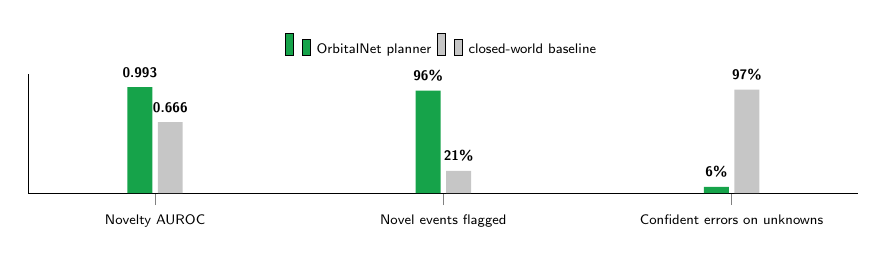
\begin{tikzpicture}
\begin{axis}[ybar,width=\columnwidth,height=3.1cm,bar width=9pt,ymin=0,ymax=1.12,axis lines*=left,ytick=\empty,
  symbolic x coords={auc,tpr,cw},xtick=data,enlarge x limits=.22,
  xticklabels={{Novelty AUROC},{Novel events flagged},{Confident errors on unknowns}},
  x tick label style={font=\tiny,align=center,text width=2.6cm},
  nodes near coords,every node near coord/.append style={font=\tiny\bfseries},
  legend style={font=\tiny,draw=none,at={(.5,1.04)},anchor=south,legend columns=2},]
\addplot[fill=grn,draw=none,point meta=explicit symbolic] coordinates
  {(auc,\vSimAucP)[\SimAucP] (tpr,\vSimTprP)[\SimTprP] (cw,\vSimCwWhP)[\SimCwWhP]};
\addplot[fill=gray!45,draw=none,point meta=explicit symbolic] coordinates
  {(auc,\vSimAucBthree)[\SimAucBthree] (tpr,\vSimTprBthree)[\SimTprBthree] (cw,\vSimCwWhBthree)[\SimCwWhBthree]};
\legend{OrbitalNet planner, closed-world baseline}
\end{axis}
\end{tikzpicture}
\end{center}
\vspace{-6pt}
{\footnotesize Higher is better for the first two, lower for the third. Simulation, preregistered held-out seeds;
on \RealNEvents{} real ZTF events the novelty AUROC is \RealCAuc{}, with certified false alarms of \ConfFa{} (bound \ConfAlphaPct).}
\end{multicols}

\vfill
\begin{tikzpicture}[remember picture,overlay]
  \fill[space] (current page.south west) rectangle ($(current page.south east)+(0,8mm)$);
  \fill[rd] ($(current page.south west)+(0,8mm)$) rectangle ($(current page.south east)+(0,8.5mm)$);
  \node[anchor=west,white!80,font=\scriptsize] at ($(current page.south west)+(11mm,4mm)$)
    {Python \textperiodcentered\ SGP4 \textperiodcentered\ Redis \textperiodcentered\ WebSockets \textperiodcentered\ Three.js/WebGL \textperiodcentered\ Streamlit \textperiodcentered\ Gaussian processes};
  \node[anchor=east,white,font=\scriptsize\bfseries] at ($(current page.south east)+(-11mm,4mm)$) {github.com/joycemalik/orbitalnet-dashboard};
\end{tikzpicture}
\end{document}
